%Sidenote from Angie: Green text after a percentage sign includes notes to the LaTeX code, useful tips and tricks I thought you might need ⁠— feel free to read them for extra info on this template.

%~~~~~~~~~~~~~~~~~~~~~~~~~~~~~~~~~~~~~~~~~~~~~~~~~~~~~~~%
% Changelog 7.21: Lab now moving from remote learning to physical laboratory, please ignore any comments after '% OLD TEXT IGNORE:'
%Changelog 10.21: Fixed the formatting of RSC referencing style 
%Changelog 1.22: Reviewed before the start of Semester 2, fixed some wording/clarification issues
%Changelog 5.22: Reviewed after semester 2, fixed some wording/clarification issues, removed OLD TEXT
%~~~~~~~~~~~~~~~~~~~~~~~~~~~~~~~~~~~~~~~~~~~~~~~~~~~~~~~%

\documentclass[twocolumn]{article} %sets the type of the document that you compile, for just now it is an article - specifically one with a two-column formatting

%~~~~~~~ Packages ~~~~~~~~~%
% Please don't be scared by the chunk of code below, these are just some handy tools that make using LaTeX easier, you can read more on your own time, for example here: https://www.latex-tutorial.com/tutorials/packages/
%\usepackage{amsmath}
% \usepackage{caption}
% \usepackage{subcaption}
\usepackage[utf8]{inputenc} %helps interpret unicode, non ASCII characters
\usepackage[T1]{fontenc} %makes font compatible with more non-ASCII characters
\usepackage[english]{babel} %allows the use of special characters and also translates some elements within the document. This package also automatically activates the appropriate hyphenation rules for the language you choose
\usepackage{ifpdf,amsmath,amsthm,amssymb,amsfonts,newtxtext,newtxmath} %helps formatting math & keeps it looking tidy when compiling PDFs
\usepackage{array,graphicx,dcolumn,multirow,abstract,hanging} %makes tables compile properly & helps with nice table formatting
\usepackage{subcaption}
\usepackage[font={it,footnotesize},labelfont=bf]{caption} %makes captions nicer
\usepackage[hyperfootnotes=false,breaklinks=true,hidelinks]{hyperref} %formats hyperlinks
%\hypersetup{colorlinks=false,} %formats hyperlinks
\usepackage{float} %improves the interface for defining floating objects such as figures and tables
\urlstyle{same} %formats urls
\usepackage{url} %formats urls
\usepackage[version=4]{mhchem} %helps format chemical formulae see more info at https://anorien.csc.warwick.ac.uk/mirrors/CTAN/macros/latex/contrib/mhchem/mhchem.pdf
\usepackage{siunitx} %formats SI units see more info at http://www.bakoma-tex.com/doc/latex/siunitx/siunitx.pdf
\usepackage{color,soul} %allows for highlighting text
\usepackage[super,sort&compress,comma]{natbib}  % use natbib
\setlength{\bibsep}{0pt plus 0.3ex} % set spacing of bibliography
\usepackage{booktabs} % \toprule \midrule \bottomrule \cmidrule(lr){a-b}
%\usepackage{capt-of}
% define centered and ragged columns:
\newcolumntype{L}[1]{>{\raggedright\arraybackslash }p{#1}} % can use m{}
\newcolumntype{C}[1]{>{\centering\arraybackslash }p{#1}}
\newcolumntype{R}[1]{>{\raggedleft\arraybackslash }p{#1}}
\newcolumntype{d}[1]{D{.}{.}{#1}} % d{3.2} for 3 places on l, 2 on r
\newcommand{\mc}{\multicolumn}
\topmargin=-.3in \oddsidemargin=-.1in \evensidemargin=-.1in \textheight=9in \textwidth=6.8in
\setlength\tabcolsep{1mm}
\setlength\columnsep{8mm}
\setlength\abovecaptionskip{.5ex}
\setlength\belowcaptionskip{.5ex}
\setlength\belowbottomsep{.3ex}
\setlength\lightrulewidth{.04em}
\renewcommand\arraystretch{1.2}
\renewcommand{\topfraction}{1}
\renewcommand{\textfraction}{0}
\renewcommand{\floatpagefraction}{.9}
\renewcommand{\thefootnote}{\roman{footnote}}
% \renewcommand{\baselinestretch}{1.00} \large\normalsize % for fixing spaces
\widowpenalty=1000
\clubpenalty=1000
\setlength{\parskip}{0ex}
\let\tempone\itemize
\let\temptwo\enditemize
\let\tempthree\enumerate
\let\tempfour\endenumerate
\renewenvironment{itemize}{\tempone\setlength{\itemsep}{0pt}}{\temptwo}
\renewenvironment{enumerate}{\tempthree\setlength{\itemsep}{0pt}}{\tempfour}
%the above is the formatting setup for keeping the two-column article and tables working nicely, feel free to tinker with it, but I suggest only doing so once you know what you're doing with LaTeX
%~~~~~~~~~~~~~~~~~~~~~~~~~~%

%!!!!!!!!!!!!!!!!!!!!!!!!!!!!!!!!!!!!!!%
% REPORT STARTS HERE %

%\date{} %if you don't want the date to show up in your report, uncomment this (=remove the percentage symbol at the start of the line)
\setcounter{page}{1} % starts counting pages from the first
\title{\textit{Experiment 6:} Lab Report Template} % change to an actual title for your report!
\author{Put Your Name Here}

\begin{document}
\twocolumn[ %this command makes your title and abstract both be one column only
\vspace{-.5in}
\maketitle
\centering
\vspace{-0.3in}
\section*{Abstract}
{\large 
A good abstract should include a clear statement of the experimental aim, some significant data points presented correctly, as well as a concise summary of trends and observations concerning your data. A great abstract will mention the specific methods used and the validity/level of error in the presnted data.

When in doubt, please consult the laboratory report guidelines available on Learn. 

}
\vspace{0.4in}
]
%\setlength{\baselineskip}{12pt plus.2pt}


\section{Introduction} % example of a heading

\textbf{Vibrational Energy}

The vibrational population can be transferred from ground state to a higher state by absorbing energies. The \textit{fundamental absorption} described the transition from v=0 to v=1, and the energy usually in range of 500 cm$^{-1}$ to 4000 cm$^{-1}$, which was within the infrared region. 

The energy levels for a diatomic molecules in an anharmonic state could be expressed as shown in equation 1.

\begin{equation}
    G(v) = (v + \frac{1}{2}) \omega_e - (v + \frac{1}{2})^2\omega_ex_e \label{eq.1}
\end{equation}

In first part of the equation 1 represented the energy of a harmonic oscillator, while the second part was the correction term for an anharmonic oscillator. The energy of anharmonic oscillator was lower than the enrgy of harmonic oscillator with a amount depend on the anharmonic constant $\omega_ex_e$. The frequency of the anharmonic oscillator was shown as $\omega_e$. With the equation 1, the ground state energy could be shown as equation 2 with v=0, and so as the first excitation state (v=1) and the second excitation state (v=2).
\begin{subequations}
    \begin{align}
        G(0) = \frac{1}{2}\omega_e - \frac{1}{4}\omega_ex_e \\
        G(1) = \frac{3}{2}\omega_e - \frac{9}{4}\omega_ex_e \\
        G(2) = \frac{5}{2}(\omega_e -\frac{25}{4}\omega_ex_e) 
    \end{align}
\end{subequations}

With equation 2, the energy of the fundamental absorption (v=0 to v=1) and the energy of the first overtone (v=0 to v=2) could be calculated as shown in equation 3. 
\begin{subequations}
    \begin{align}
        G(0 \rightarrow 1) = G(1) - G(0) = \omega_e - 2\omega_ex_e \\
        G(0 \rightarrow 2) = G(2) - G(0) = 2(\omega_e - 3\omega_ex_e) 
    \end{align}
\end{subequations}

\textbf{Rotational Energy}

The rotational energy could be described using equation 4 for a diatomic molecule.

\begin{equation}
    F(J) = B_v(J + 1) \label{eq.4}
\end{equation}

In this equation, $J$ was the rotational quantum number, while $B_v$ was the rotational constant, which was related to the moment of inertia $I$ as shown in equation 5. 

\begin{subequations}
    \begin{align}
        B_v = \frac{h}{8\pi^2cI} \\
        I = \mu r^2
    \end{align}
\end{subequations}



\textbf{Transition Energy}

Since the vibrational transition and the vibrational transition involved two very different frequencies. The energy for vibrational rotational transition could be expressed as equation 6, while the centrifugal distortion was ignored here. 

\begin{equation}
    S(v,J) = (v + \frac{1}{2}) \omega_e - (v + \frac{1}{2})^2\omega_ex_e + B_v(J + 1) 
\end{equation}

\hl{The scale of the constant B would change with increasing vibrational state. }




\textbf{Rotational Selection Rules}
%The transition where $\delta J = 0$ was forbidden, meaning that transition from $J=1 \rightarrow J' = 1$ was not allowed. For $\delta J = 1 $ was allowed and would be shown in the spectrum. The P, Q, R branches were defined based on $\delta J$:

\begin{enumerate}
    \item P branch - A transition where J=-1
    \item Q branch - A transition where J=0
    \item R branch - A transition where J=+1
\end{enumerate}

\textbf{The Q branch usually would not appeared in the spectrum because it was forbidden (photon unit energy). 
However, it could appear in the spectrum when ...}




\section{Methodology}

The 10 $cm^3$ gas cell was flushed with nitrogen and sealed with the Teflon lids. The background scan was performed with this cell using \textbf{FT-IR spectrometer} in the range 6000 cm$^{-1}$ - 2000 cm$^{-1}$ for \textbf{64 folds with resolution as 0.5}. Three drops of concentrated HCl was added into the cell, and the spectrum was recorded under the same conditions. 

The background scan was performed again under the same conditions with a larger gas cell. Cigarette smoke was captured in the cell. The spectrum of cigarette smoke was recorded under the same conditions. 



\section{Results}  

The IR sepctrum of HCl was recorded. The fundamental absorption was observed at 2880 cm$^{-1}$ as shown in Figure 1, while the first overtone was observed at 5760 cm$^{-1}$ as shown in Figure 2. 

\begin{figure}[h!]
    \begin{subfigure}[b]{0.95\columnwidth}
        %\centering
        \caption{1a}
        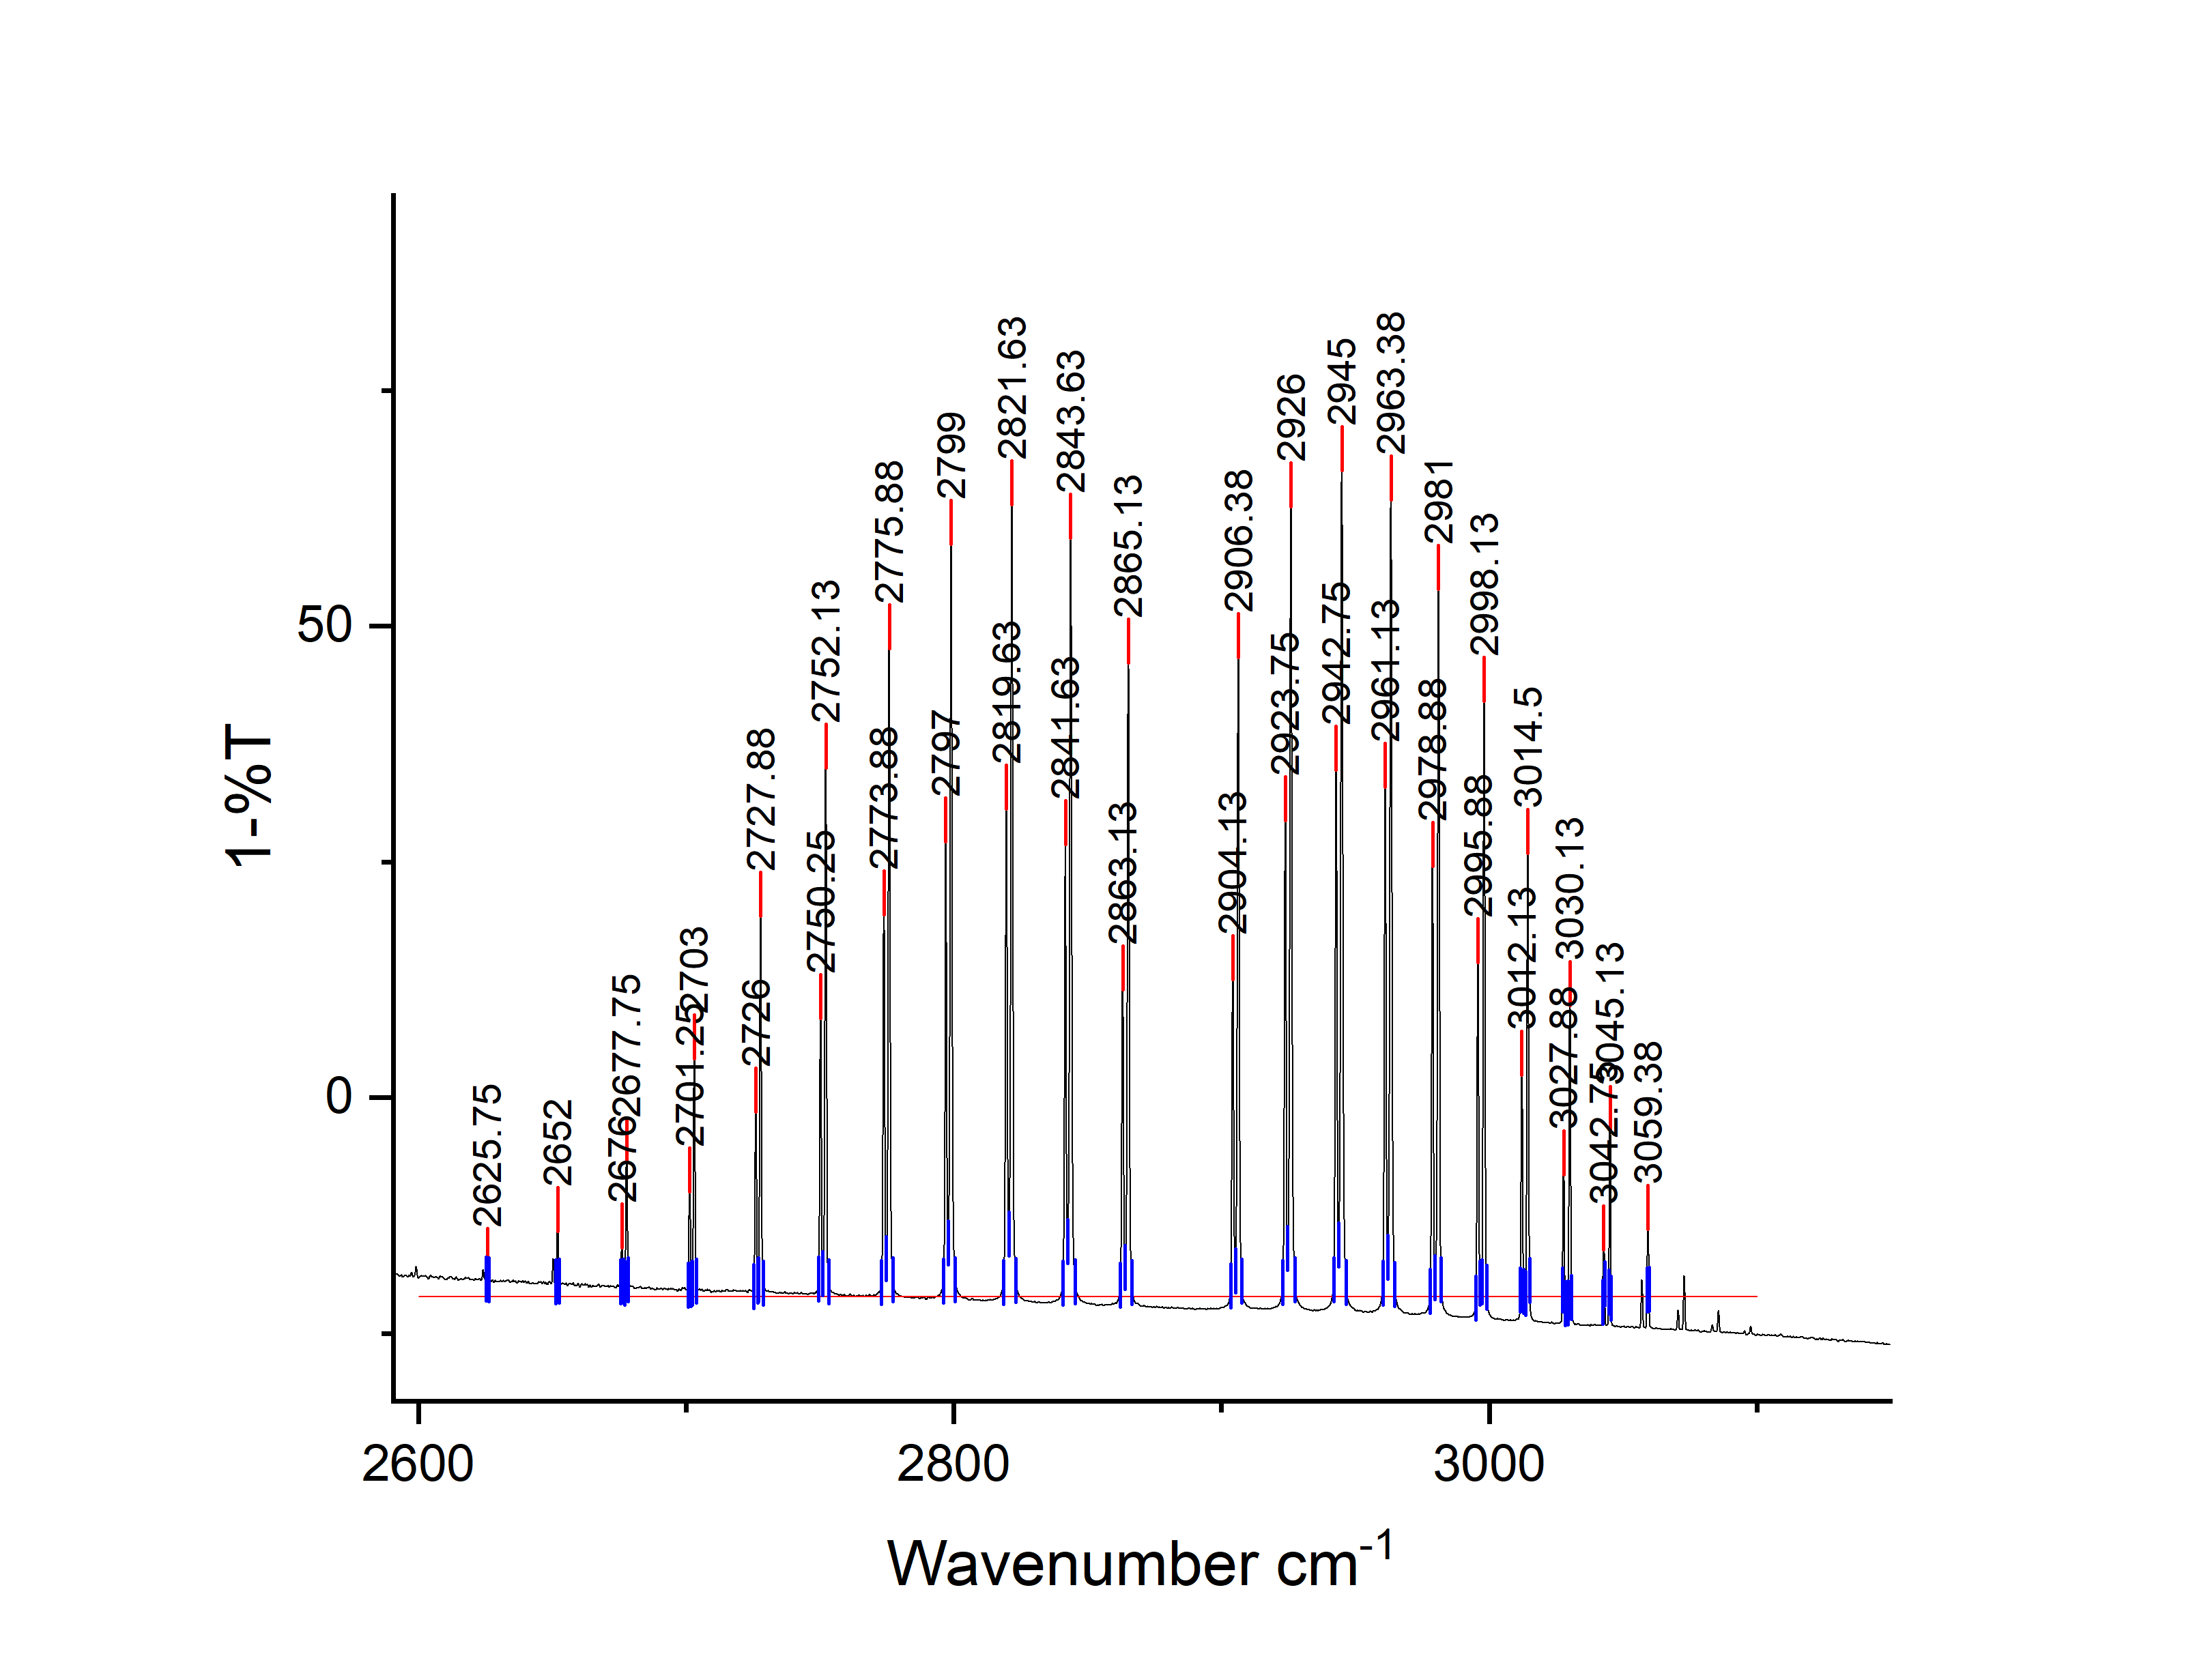
\includegraphics[width=\columnwidth]{HCl fund.png}
        %\caption{1a}
        \label{fig:sfig1}
    \end{subfigure}
    \begin{subfigure}[b]{0.95\columnwidth}
      %\centering
      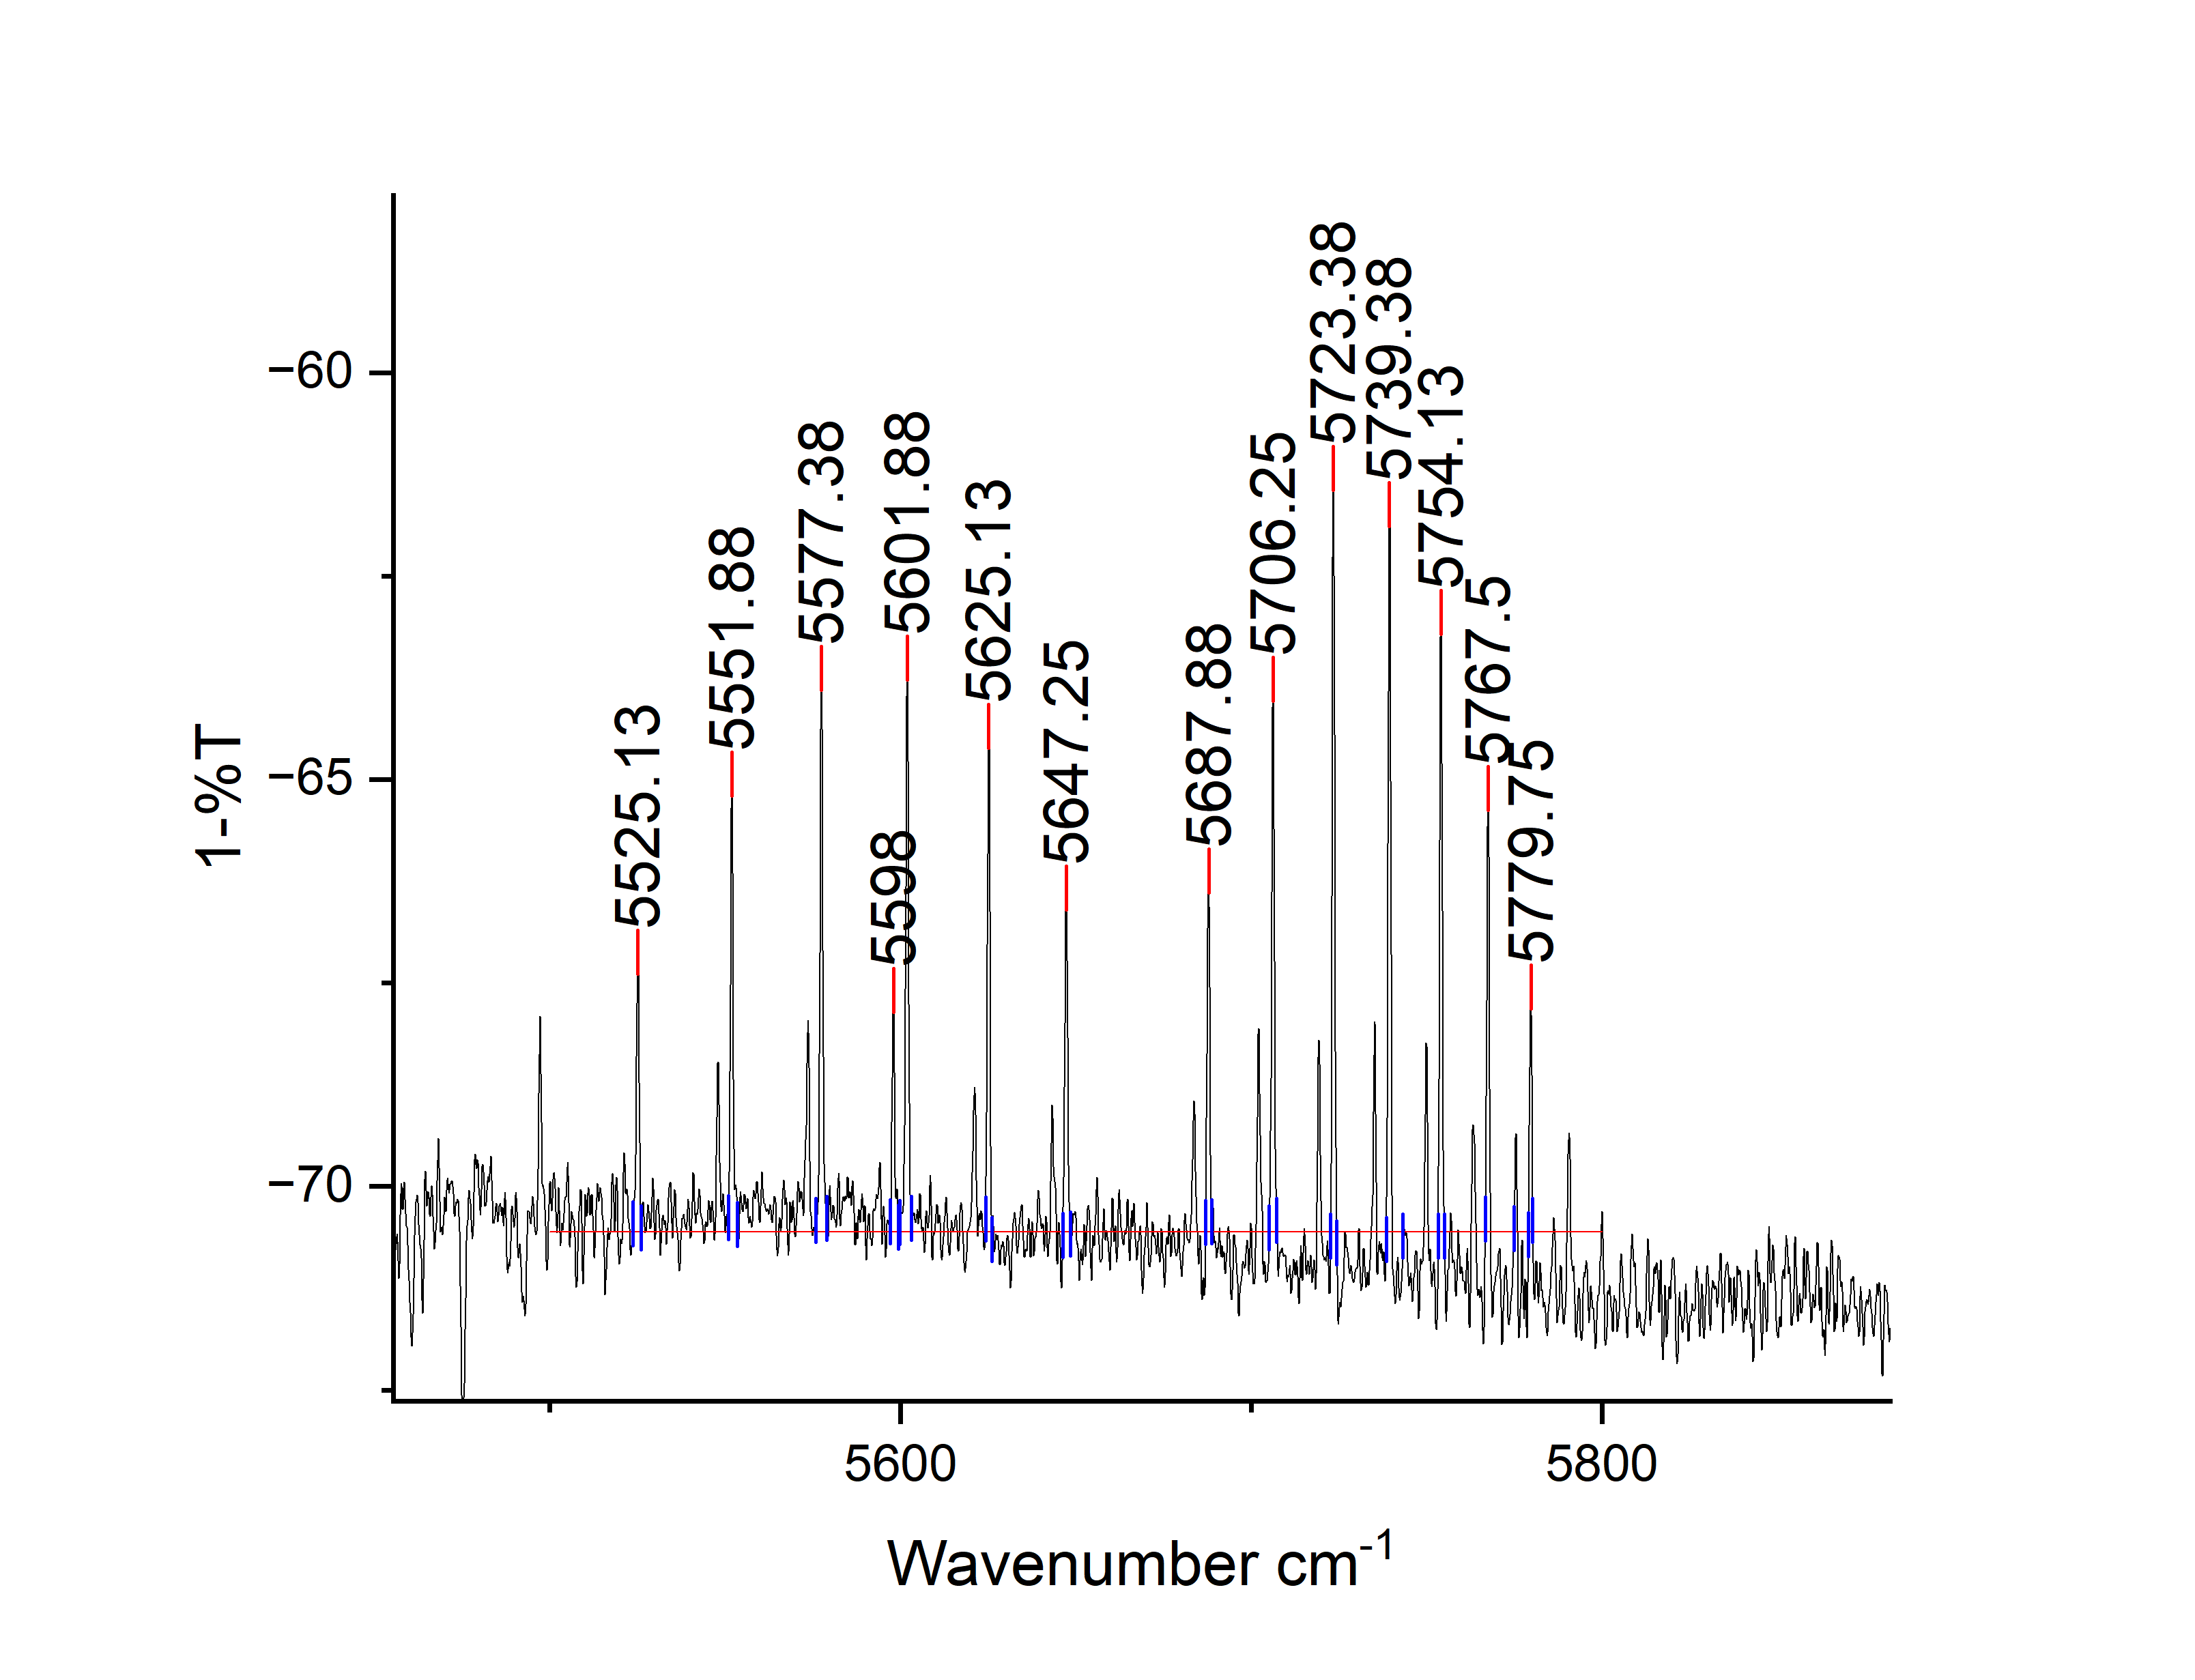
\includegraphics[width=\columnwidth]{HCl over.png}
      \caption{1b}
      \label{fig:sfig2}
    \end{subfigure}
    \caption{plots of....}
    %\label{fig:fig}
\end{figure}

\textbf{The trends; identify the P, Q, R branches in the spectrum. }

The wavenumber of the fundamental absorption for HCl$^{35}$ and HCl$^{37}$ were recorded separately in Table 1 and Table 2. The value of R(J)-P(J) and R(J)-P(J+2) were calculated to determine the rotational constant $B_0$ and $B_1$ for HCl$^{35}$ and HCl$^{37}$ respectively as shwon in Table 1 and Table 2.

\begin{table}[h]
    \caption{The wavenumber of the fundamental absorption for HCl$^{35}$ in P branch and R branch.}
    \begin{tabular}{L{.1in}C{.7in}C{.7in}C{.7in}C{.8in}}\toprule
        J & P (cm$^{-1}$)      & R     (cm$^{-1}$)  & R(J)-P(J) (cm$^{-1}$)& R(J)-P(J+2) (cm$^{-1}$)\\\midrule
        0 &     -   & 2906.38 &     -     & 62.75       \\
        1 & 2865.13 & 2926.00 & 60.87     & 104.37      \\
        2 & 2843.63 & 2945.00 & 101.37    & 146.00      \\
        3 & 2821.63 & 2963.38 & 141.75    & 187.50      \\
        4 & 2799.00 & 2981.00 & 182.00    & 228.87      \\
        5 & 2775.88 & 2998.13 & 222.25    & 270.25      \\
        6 & 2752.13 & 3014.50 & 262.37    & 311.50      \\
        7 & 2727.88 & 3030.13 & 302.25    & 352.38      \\
        8 & 2703.00 & 3045.13 & 342.13    &   -          \\
        9 & 2677.75 &     -   &    -      &    - \\\bottomrule
   \end{tabular}
\end{table}

\begin{table}[h]
    \caption{The wavenumber of the fundamental absorption for HCl$^{37}$ in P branch and R branch.}
    \begin{tabular}{L{.1in}C{.7in}C{.7in}C{.7in}C{.8in}}\toprule
        J & P (cm$^{-1}$)      & R     (cm$^{-1}$)  & R(J)-P(J) (cm$^{-1}$)& R(J)-P(J+2) (cm$^{-1}$)\\\midrule
        0 & - & 2904.13 &       -   & 62.50       \\
        1 & 2863.13 & 2923.75 & 60.62     & 104.12      \\
        2 & 2841.63 & 2942.75 & 101.12    & 145.75      \\
        3 & 2819.63 & 2961.13 & 141.50    & 187.25      \\
        4 & 2797.00 & 2978.88 & 181.88    & 228.63      \\
        5 & 2773.88 & 2995.88 & 222.00    & 269.88      \\
        6 & 2750.25 & 3012.13 & 261.88    & 310.88      \\
        7 & 2726.00 & 3027.88 & 301.88    & 351.88      \\
        8 & 2701.25 & 3042.75 & 341.50    &    -    \\
        9 & 2676.00 &     -   &    -      &    - \\\bottomrule
    \end{tabular}
\end{table}

The rotational constant $B_0$ could be obtained by ploting the R(J)-P(J) against (J+1/2) based on \hl{equation x} as shown in Figure 3(a) for HCl$^{35}$. The rotational constant $B_1$ could be obtained by ploting the R(J)-P(J+2) against (J+3/2) based on \hl{equation x}as shown in Figure 3(b) for HCl$^{35}$.

\begin{figure}[h!]
    \begin{subfigure}[b]{0.95\columnwidth}
        %\centering
        \caption{1a}
        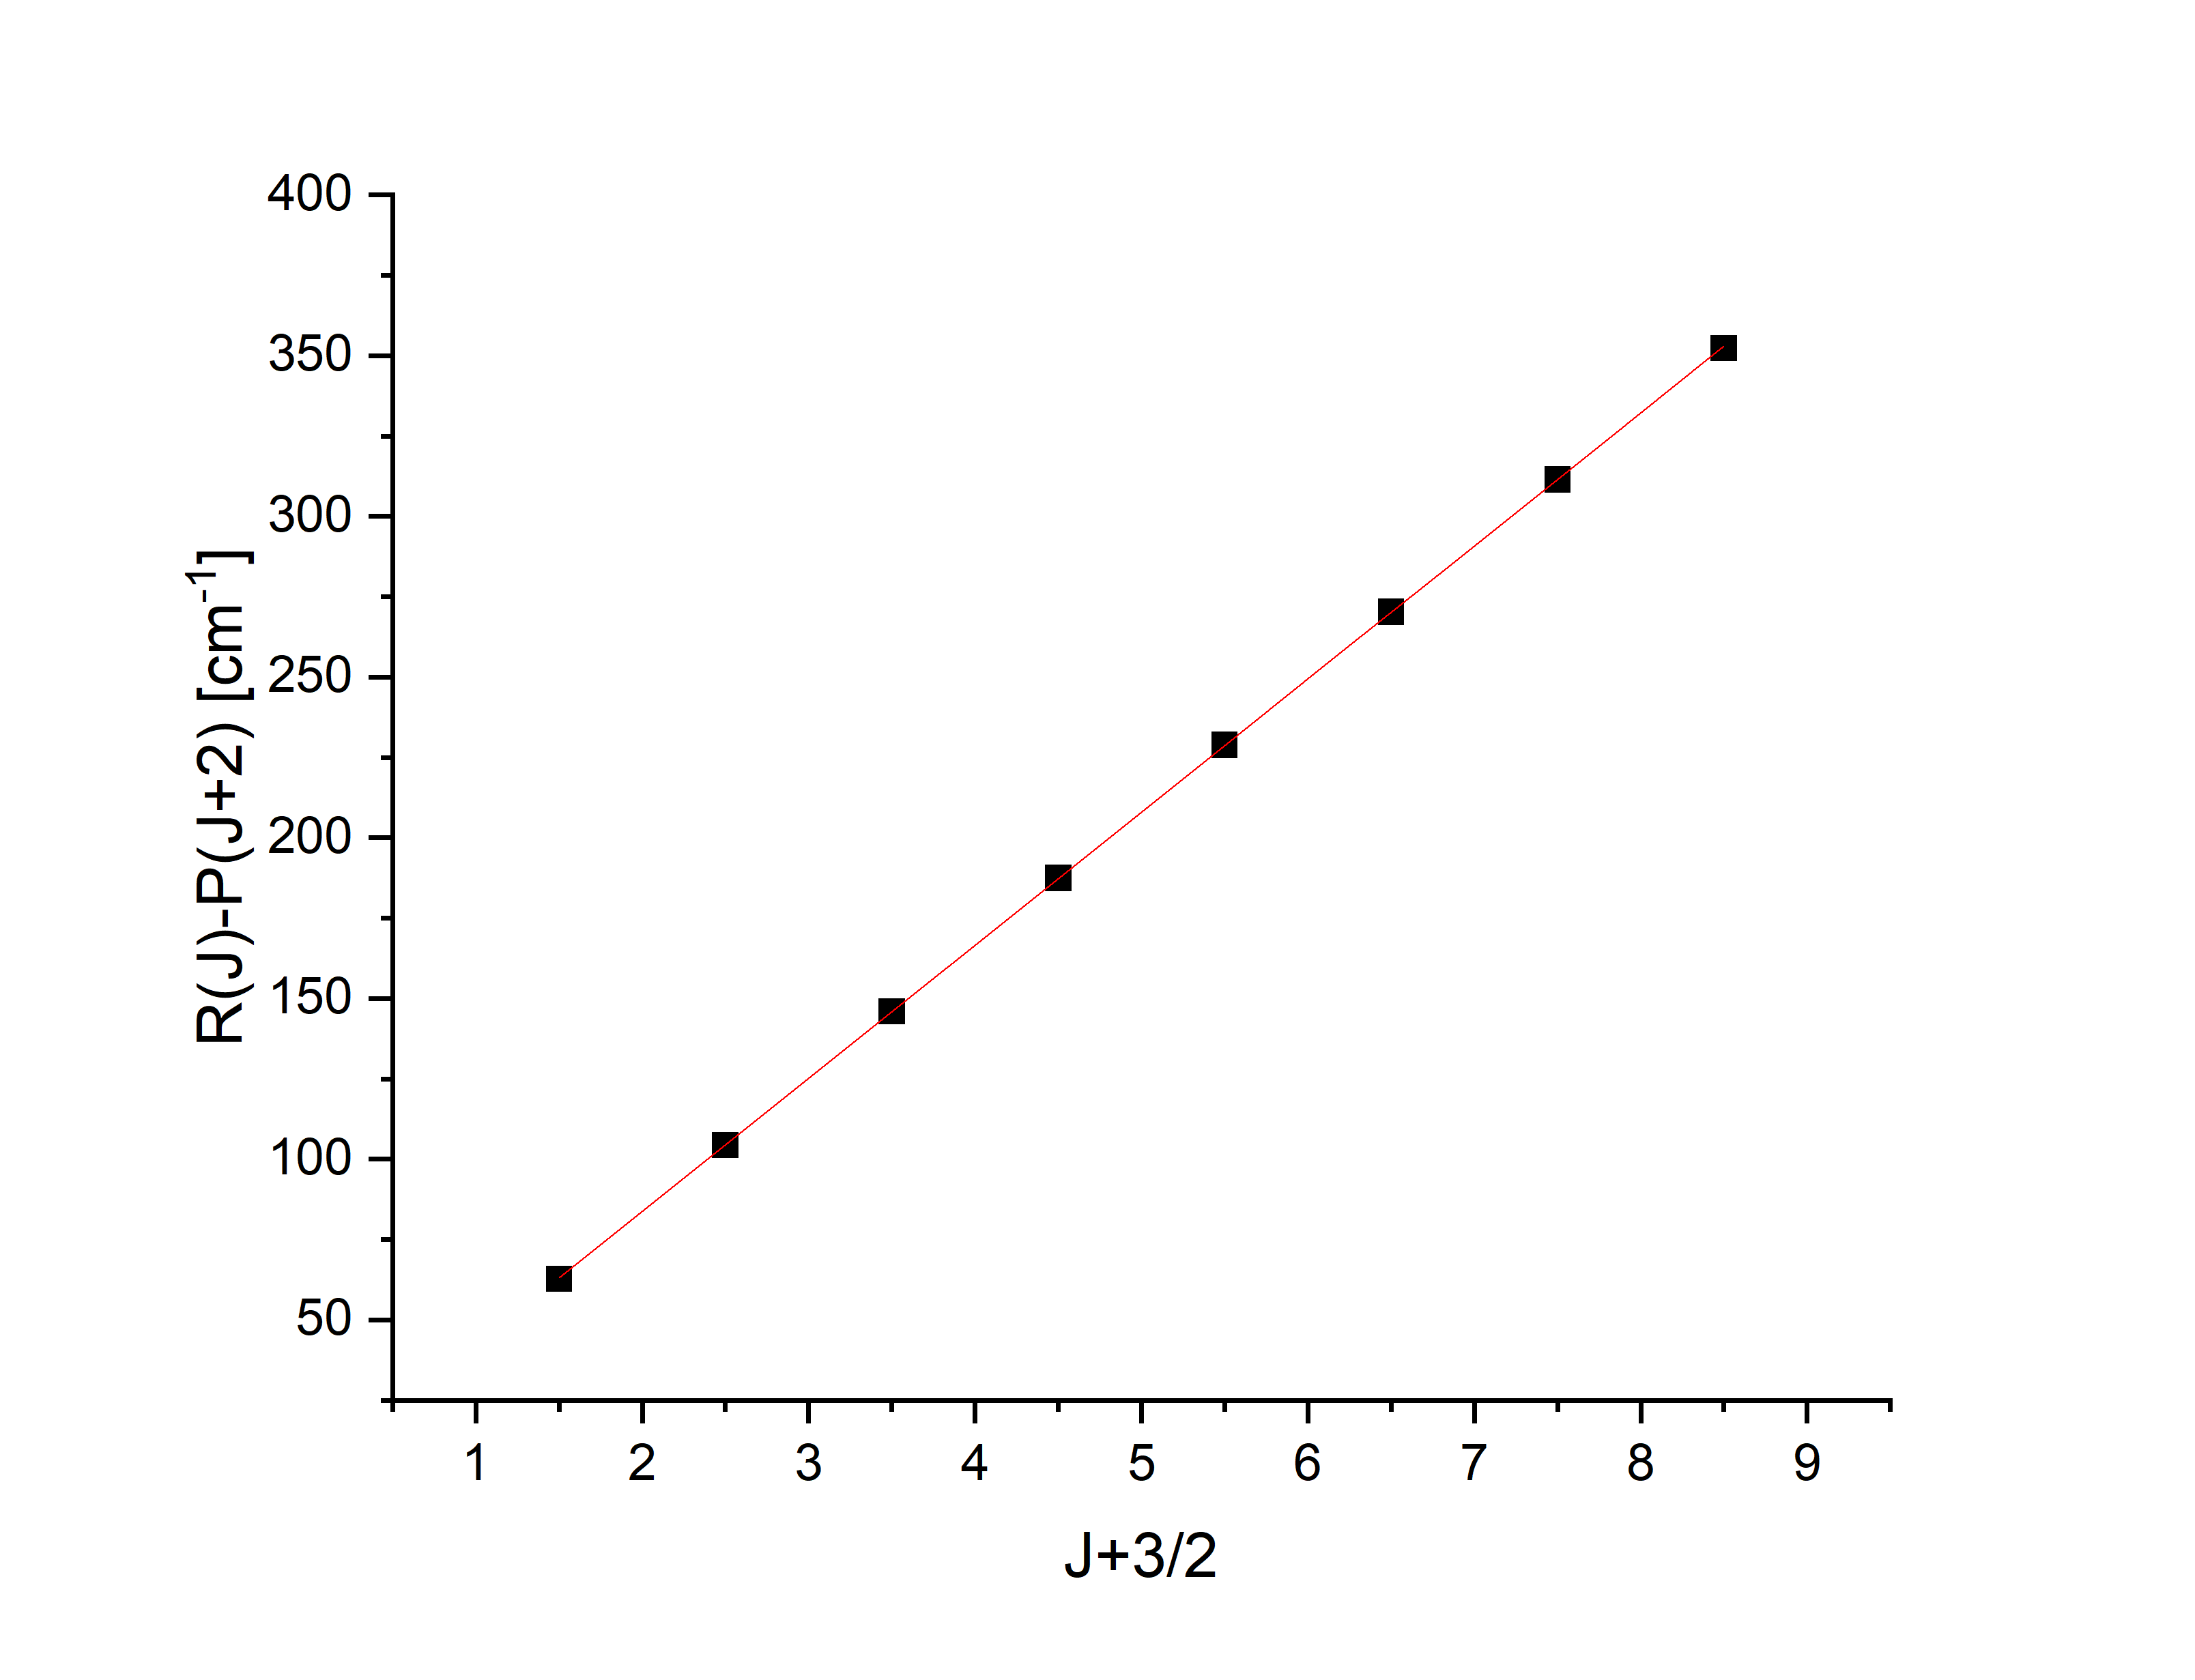
\includegraphics[width=\columnwidth]{HCl-35-B0.png}
        %\caption{1a}
        \label{fig:sfig1}
    \end{subfigure}
    \begin{subfigure}[b]{0.95\columnwidth}
      %\centering
      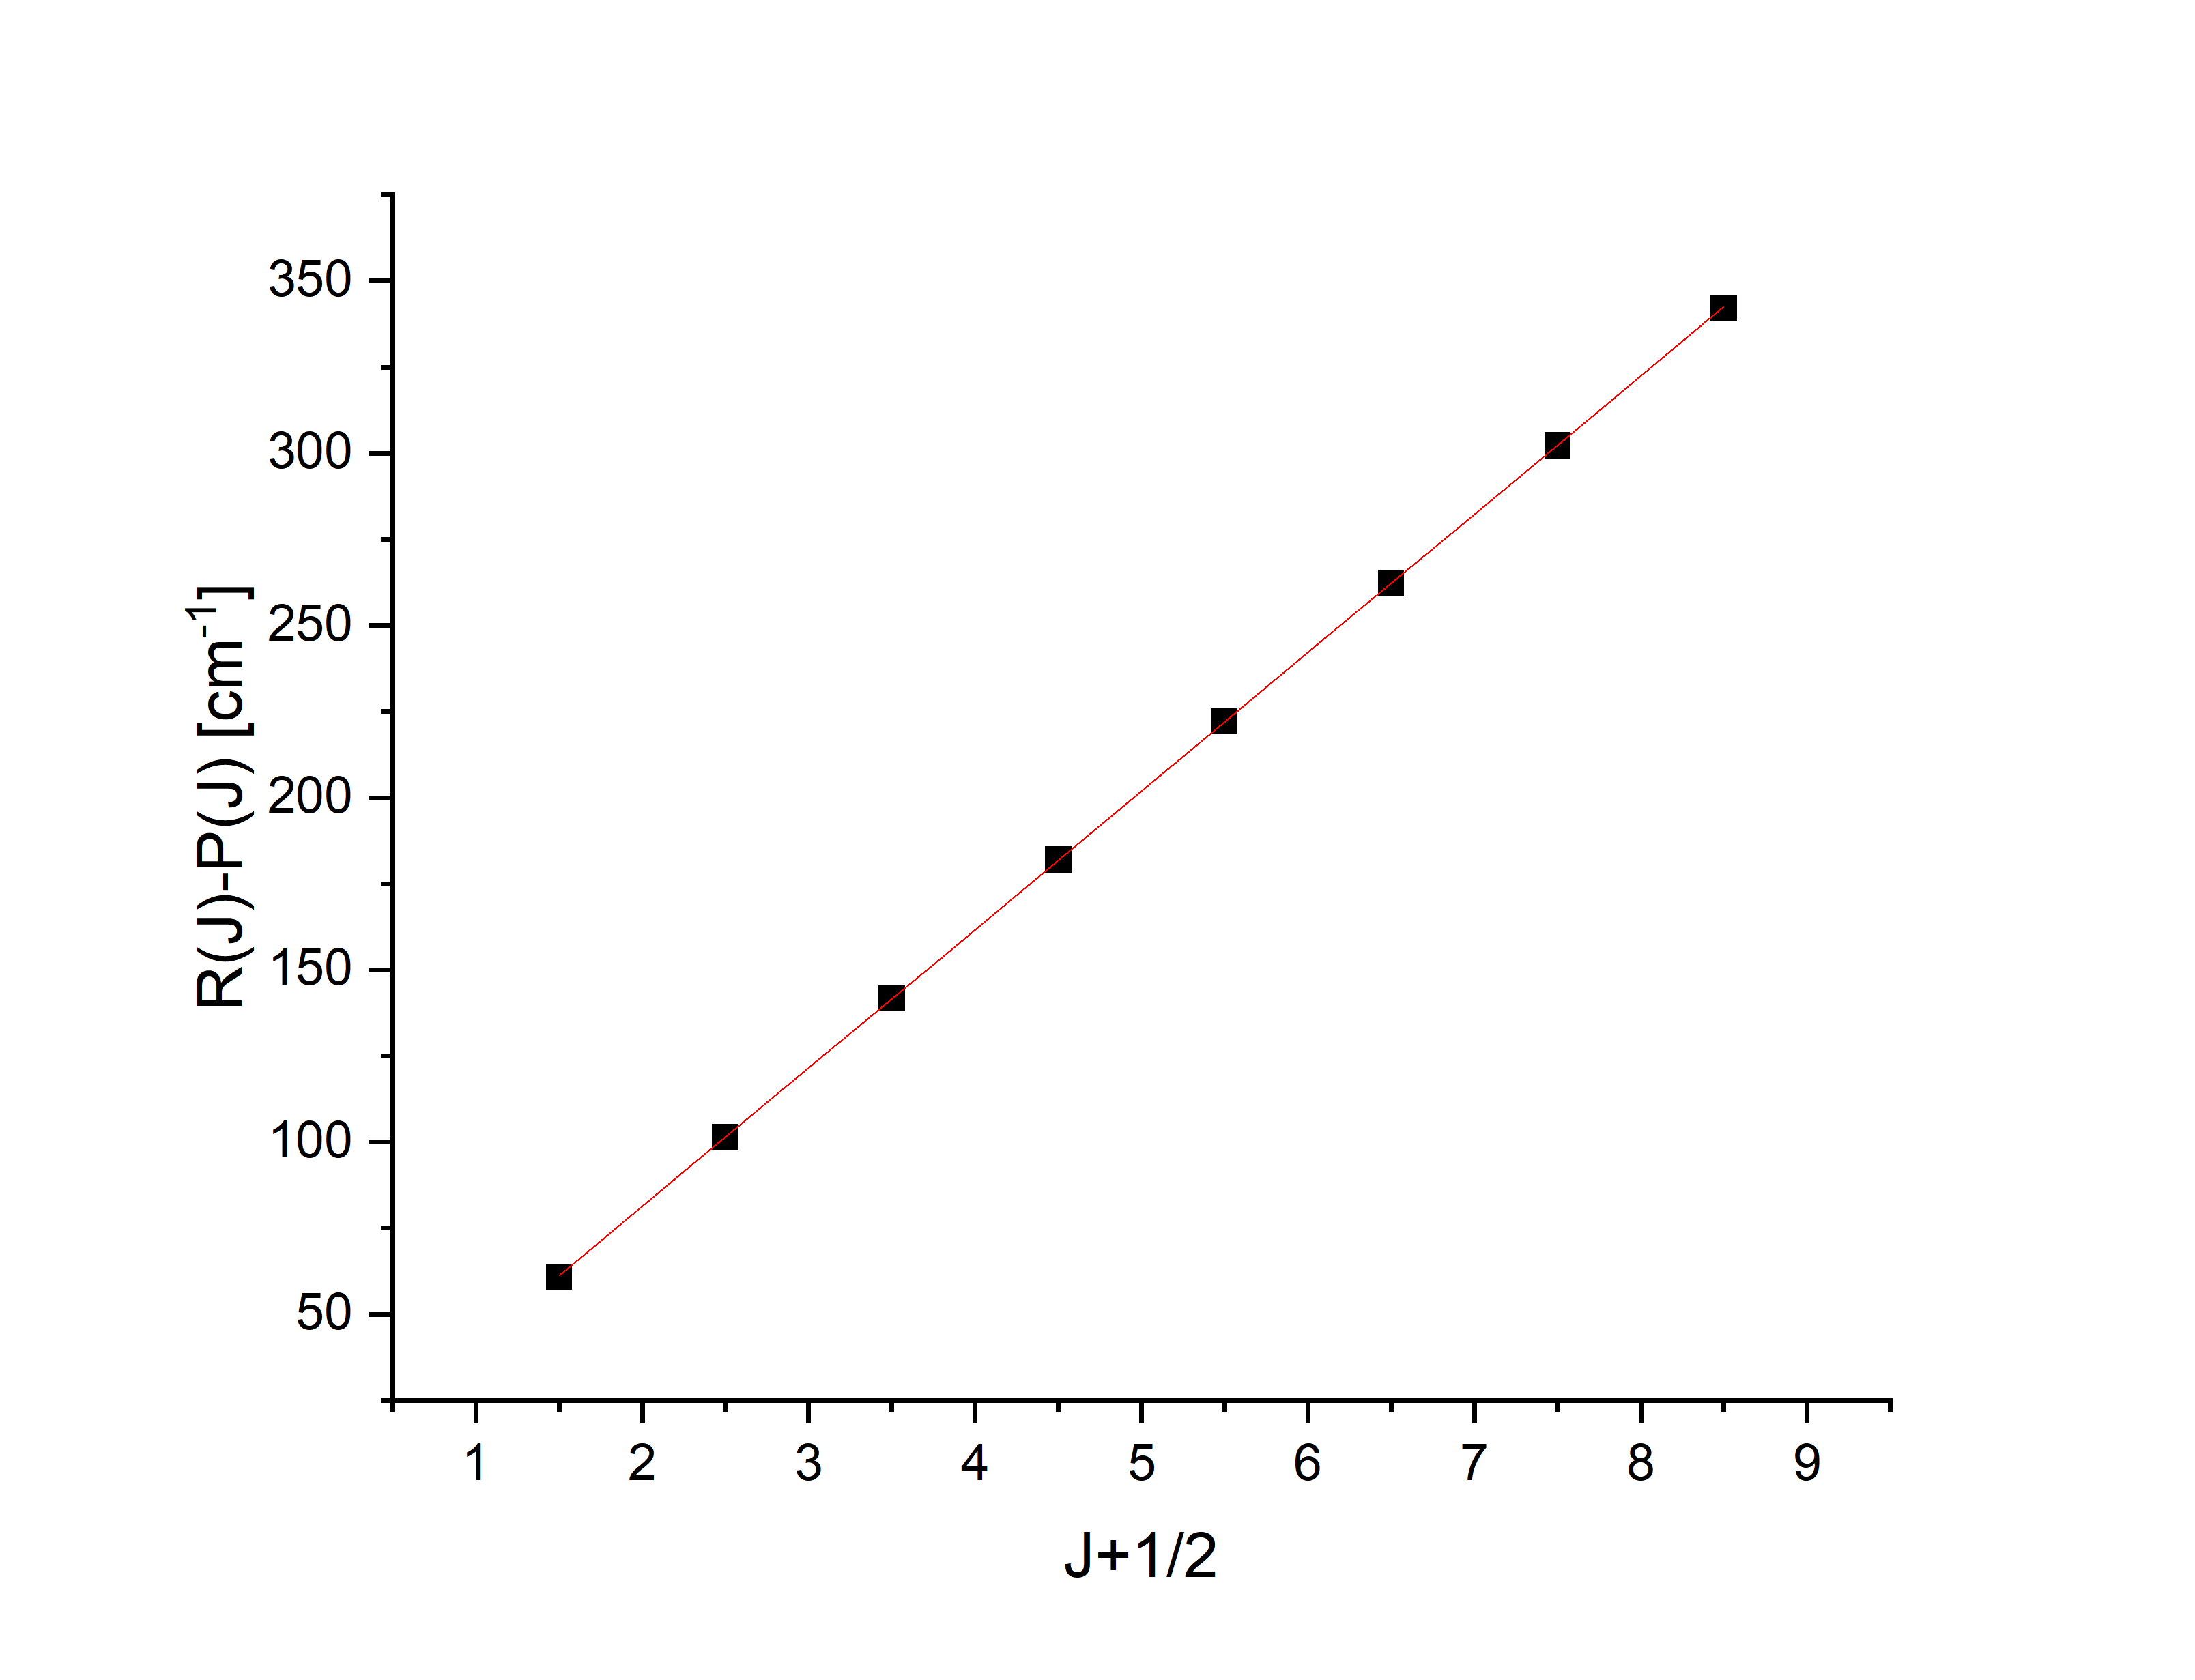
\includegraphics[width=\columnwidth]{HCl-35-B1.png}
      \caption{1b}
      \label{fig:sfig2}
    \end{subfigure}
    \caption{plots of....}
    %\label{fig:fig}
\end{figure}

The slope in Figure 3(a) was 41.3950\hl{$\pm$ error}, which was four times the rotational constant $B_0$, which was calculated as shown in \hl{equation x}.
\begin{equation}
    B_0 = \frac{41.3950}{4} = 10.3488  cm^{-1}
\end{equation}

The slope in Figure 3(b) was 40.1825\hl{+- error}, which was four times the rotational constant $B_1$, which was calculated as shown in \hl{equation x}.
\begin{equation}
    B_1 = \frac{40.1825}{4} = 10.0456  cm^{-1}
\end{equation}

The \hl{rotational constant $B_e$} could be calculated based on $B_0$ and $B_1$ as shown in \hl{equation x} based on \hl{equation x}.

\begin{subequations}
    \begin{align}
        10.3488 = B_e - \alpha_e (0+1/2)\\
        10.0456 = B_e - \alpha_e (1+1/2)
    \end{align}
\end{subequations}

The value of $B_e$ was determined by solving these two equations, which was 10.5003 $cm^{-1}$. The value of $\alpha_e$ was also obtained as 0.3029 $cm^{-1}$.

The bond length of HCl in different vibrational could be caluclated using $B_0$, $B_1$, and $B_e$ based on \hl{equation 5(a)} and \hl{equation 5(b)} respectively as shown in \hl{equation x}. 


\begin{subequations}
    \begin{gather}
        %r =\sqrt{(\frac{h}{8\pi^2\mu B c})}\\
        \mu = \frac{m_H m_{^{35}Cl}}{m_{H}+m_{^{35}Cl}} = 1.6273 \times 10^{-25} kg\\
        r_0 = \sqrt{(\frac{h}{8\pi^2\mu B_0 c})}\\
        r_1 = \sqrt{(\frac{h}{8\pi^2\mu B_1 c})}\\
        r_e = \sqrt{(\frac{h}{8\pi^2\mu B_e c})}
    \end{gather}
\end{subequations}


The equilibrium oscillator frequency $\omega_e$ and the anharmonic constant $x_e$could be calculated based on the energy of the fundamental absorption and the first overtone as shown in \hl{equation 3}. The frequency of the fundamental absorption was 2885.76 cm$^{-1}$, while the frequency of the first overtone was 5667.57 cm$^{-1}$. The value of $\omega_e$ and $x_e$ were calculated as shown in \hl{equation x}.

\begin{subequations}
    \begin{gather}
        2885.76 = \omega_e - 2\omega_ex_e \\
        5667.57 = 2(\omega_e - 3\omega_ex_e)\\
        \omega_e = 2989.70 cm^{-1}\\
        \omega_e x_e = 51.9725 cm^{-1}\\
        x_e = 0.0017384
    \end{gather}
\end{subequations}

The zero point energy of HCl$^{35}$ could be calcualted using equation 2(a) with the value of $\omega_e$ and $x_e$ as shown in \hl{equation x}. 

\begin{equation}
    G(0) = \frac{1}{2}\omega_e - \frac{1}{4}\omega_ex_e = 1494.86 cm^{-1}
\end{equation}

The force constant of HCl$^{35}$ bond could be calculated as shown in \hl{equation x} and the reduced mass ($\mu$) of HCl$^{35}$ was calculated as 1.6273 $\times$ 10$^{-25}$. 

\begin{subequations}
    \begin{gather}
        v = \frac{1}{2\pi}\sqrt{\frac{k}{\mu}} = 2885.76 cm^{-1}\\
        k = \mu v^2 (2\pi)^2 = 1.0001 \times 10^{3} Nm^{-1}
    \end{gather}
\end{subequations}

The value of $B_0$, $B_1$, $B_e$,$\alpha_e$, $r_0$,$r_1$, $r_e$, $\omega_e$, $x_e$, $G(0)$, and $k$ for HCl$^{35}$ were summaried and for HCl$^{37}$ were calculated using the same method as shown in Table 3. This value was compared with the literature value.

\begin{table}[h]
    \caption{The value of $B_0$, $B_1$, $B_e$,$\alpha_e$, $r_0$,$r_1$, $r_e$, $\omega_e$, $x_e$, $G(0)$, and $k$ for HCl$^{35}$ and HCl$^{37}$.}
    \begin{tabular}{L{.7in}C{.7in}C{.7in}C{.7in}}\toprule
          & HCl$^{35}$& HCl$^{37} $& Literature value \\\midrule
        $B_0$ (cm$^{-1}$)& 10.3488 &  &\\
        $B_1$ (cm$^{-1}$)& 10.0456 &  &\\
        $B_e$ (cm$^{-1}$)& 10.5003 &  &\\
        $\alpha_e$ (cm$^{-1}$)& 0.3029 &  &\\
        $r_0$ (pm)& 127.9 &  &\\
        $r_1$ (pm)& 128.9 &  &\\
        $r_e$ (pm)& 128.4 &  &\\
        $\omega_e$ (cm$^{-1}$)& 2989.70 &  &\\
        $x_e$ & 0.0017384 &  &\\
        $G(0)$ (cm$^{-1}$)& 1494.86 &  &\\
        $k$ (Nm$^{-1}$)& 1.0001 $\times$ 10$^{3}$ &  &\\\bottomrule
    \end{tabular}
\end{table}

The IR spectrum of the cigarette was recorded as shown in Figure \ref{cigall}.

\begin{figure}[h!]
    \centering
    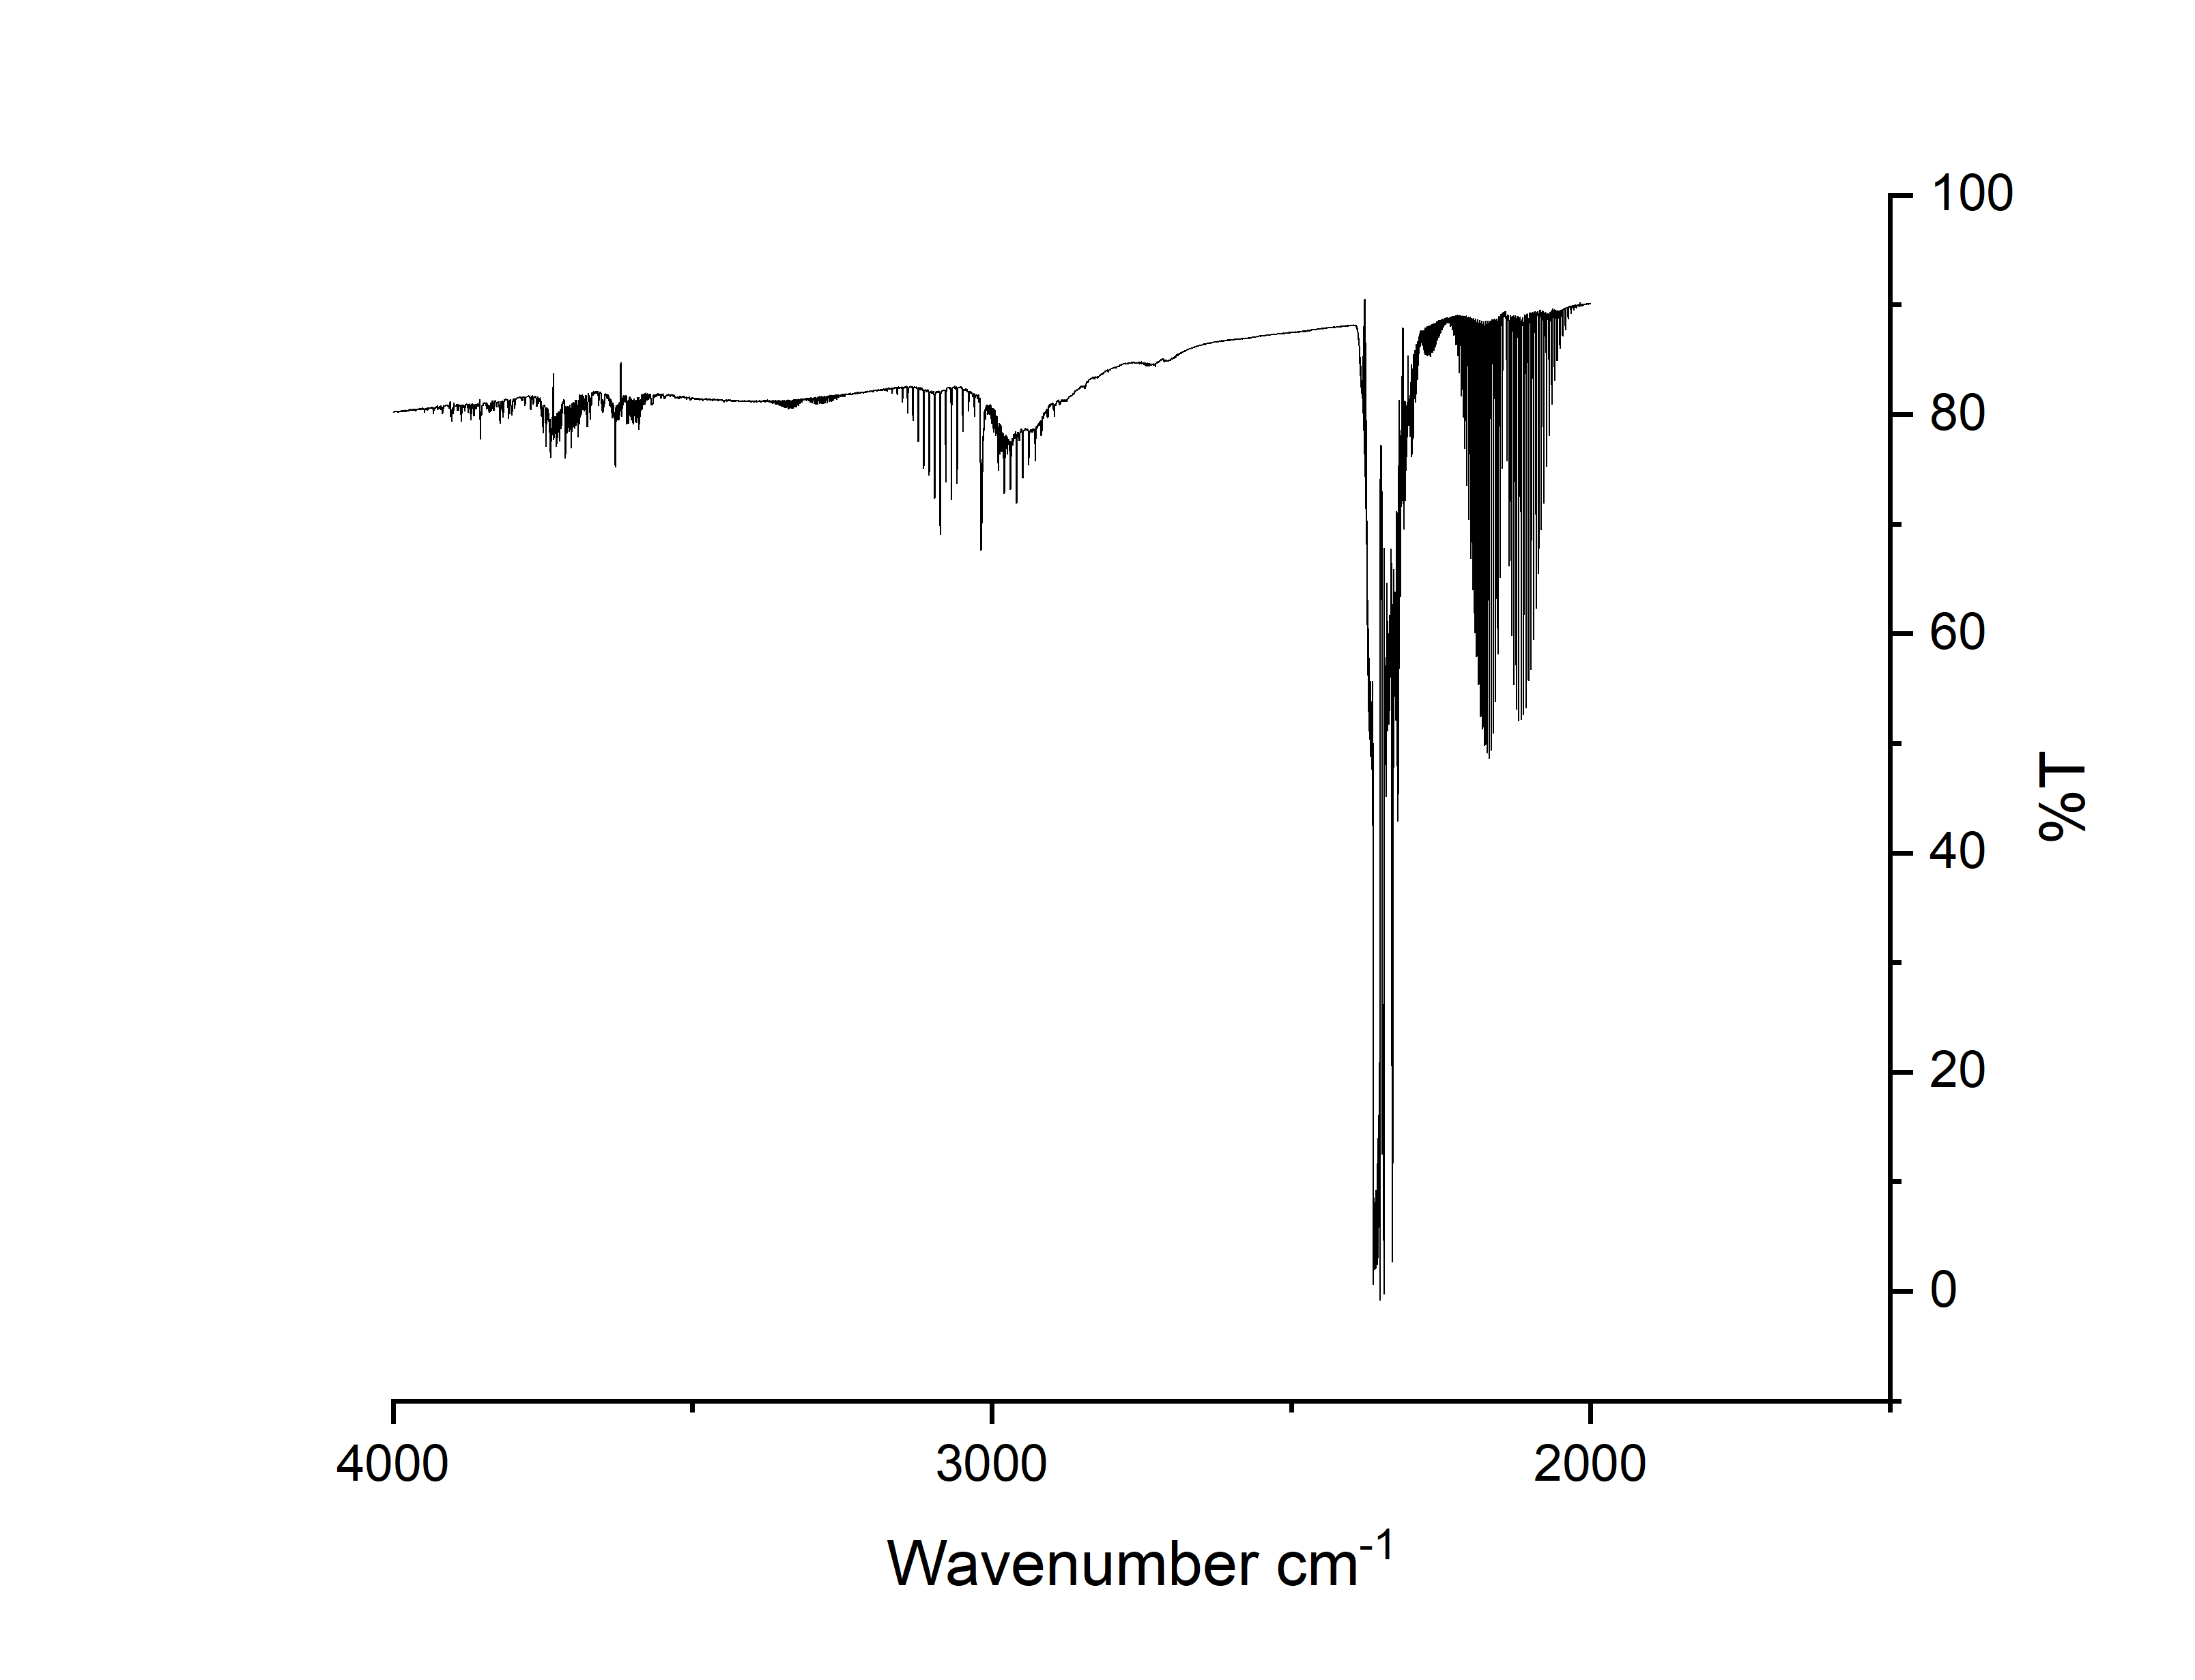
\includegraphics[width=\columnwidth]{Cig-all.png}
    \caption{The IR spectrum of the cigarette.}
    \label{cigall}
\end{figure}






% The results section should contain \textbf{all} the relevant experimental data that you collected.

%  %Here is an example of a table.
%  \begin{table}[h] %the [h] here instructs the table to assume a particular position on the page, read more on table positioning here: https://www.overleaf.com/learn/latex/Positioning_images_and_tables if your tables aren't positioned as you wish them to be, try experimenting with different parameters in the square brackets
%  \caption{Good header, or caption, makes the table or figure self-contained, it should provide enough information so that the table or figure could be understood on its own, without the main text.}
%  \begin{tabular}{L{.7in}C{.7in}C{.7in}C{.7in}}\toprule
%   & column 1 \textit{is really long} & column 2 & column 3\\\midrule
%  Line 1 & 68.28 & 45.30 & 56.79 \\
%  Line 2 & 54.06 & 38.63 & 46.35 \\\midrule %this is just an example on how to include an extra line, you can remove it if you do not need it
%  Line 3 & 61.17 & 41.97 & \\\bottomrule
%  \end{tabular}
%  \end{table}
%  %Be mindful that LaTeX -- unlike MS Word/Open Office/etc. -- does not allow for tables breaking across a page, by default. If the table is too big to fit into the remaining space of a page/column, it will instead be moved to the top of the following page/column. The resulting "empty" space will be filled with text, even if the text belongs to a different section! There are ways to prevent this, if you wish, but you may have to Google/look up how table formatting works :)

% Please organize the data in a logical manner, as this will make referencing from your discussion section much easier. You can see an example of what a table should look like in Table 1. Be mindful of formatting and presentation of both tables and figures; always consider the inclusion of textual cues, the placement of captions, correct units, overall appearance, and logical placement. Make sure your figures have good resolution! Grainy, unfocused, or otherwise shabby figures will lead to point deduction. Be careful about referencing, any literature data you use in your tables or figures needs to be cited. If you take a figure from a certain literature source, you need to \textbf{explicitly} reference it as such! Even if you make your own figures in ChemDraw or other software, if they are similar to or otherwise use ideas from a literature source, you must cite this appropriately.

%  Please make sure you describe the data, particularly any trends that are apparent -- always avoid data-dumps. The best result section will guide the reader through the data, pointing out any important trends, values, or possible errors.

%  \bigskip %this is a way to force LaTeX into inserting a blank line/space, can be small, medium, or fixed by instead using the '\vspace' command!

%  If you wish to learn more about how to format tables, please visit \href{https://es.overleaf.com/learn/latex/Tables}{\textbf{this page}}.
%  You can also find a handy tool which can generate tables for you here: \url{https://www.tablesgenerator.com/}




\section{Discussion}

%  The ideal discussion will provide \textbf{full justification} of all the trends presented in the results section. 
%  Be sure to include complete reasoning for \textbf{why} the trends appear, make use of your knowledge of chemistry and concepts you explained in the introduction.
%  Reference the data tables from the results' section as necessary. 
%  %Here is an example of a figure.
%  \begin{figure}[h!]
%  \centering
%  \includegraphics[width=0.95\columnwidth]{figures/example.png} %an example of how to make your figure a specific size (fraction of the width of the column), if you'd like it to span the column instead, delete the number before the \)
%  \vspace{2mm} %just an example of how space can be added if need be, replace with '\hspace' for horizontal padding
%  \caption{Same as with table headers applies here. Please note that while in tables the caption is placed above, with figures the caption should be placed below.}
%  \end{figure}

%  Make use of figures and/or external references to support your discussion points. An example figure is shown above as Figure 1.

%  The best discussion will also include a brief paragraph with conclusions (for each part of the experiment) and future work. Future work, in this case, refers to a brief discussion on the validity of your chosen method, and the justification of using computational methods for the purposes of this experiment. The best discussion will offer some suggestions on the improvement of the experimental design.

%  \textbf{Please use concise and scientific tone in your writing. Academic writing, by convention, uses the past tense and a passive voice. Try to emulate the style you see in textbooks/papers. Avoid the use of first (I/we) or second (you) person, informal language, overuse of conjunctions and pronouns (especially 'this/that'). Make sure to proofread and spellcheck your work before submitting!}

%  Again, if you aren't sure what is appropriate for academic writing, please consult the many guides available online, such as \href{https://libguides.reading.ac.uk/writing/style}{\textbf{this one}}





\section{Investigation Question}

this is a citation \cite{Example}
% Please include the write-up to your investigation question here. Include any relevant figures, sources, or background information, as instructed in your manual.
% \\
% The best Investigation Question will include:
% \\1) a short, relevant introduction to the problem,
% \\2) a clear and well-worded proposal of a solution (hypothesis), and 
% \\3) a concise and well-researched backing/explanation for the solution. 

% Use appropriate scientific language and make sure to properly reference all of your sources!

% \vspace{8mm}
% \hrule

% %% THE FOLLOWING SECTIONS CONTAIN SOME ADDITIONAL INFORMATION FOR YOUR CONVENIENCE, MAKE SURE TO REMOVE THEM FROM YOUR OWN REPORT %%

% \section*{Note on the Citation} %Delete this section in your own report
% All sources should be formatted in the Royal Society of Chemistry (RSC) referencing style \cite{Example}. If you don't know what this means, I strongly recommend reviewing how citation and referencing works in general, and looking into the style guides for the RSC style in particular. 
% %more info at https://edu.rsc.org/download?ac=14556  

% If you use a different referencing style (MLA, Harward, etc.) please indicate so in a footnote\footnote{Example on how to format a footnote in \LaTeX{}} of your citation section, so that the demonstrator marking your work knows that you've used something different and can check it for errors!

% With Overleaf, you can simply import a .bib file into your file tree (the panel on the left-most side of your screen) and the bibliography command will automatically compile them for you. Please make sure to include relevant in-text references using the \textbackslash cite command.
% The \textbackslash printbibliography command will then generate the proper references section for you!

% .bib file can be easily obtained using a reference-management software. If you don't know what this is, or don't yet use one, I \textbf{strongly} recommend looking into one! Personally, I use \href{https://www.mendeley.com/reference-management/reference-manager}{Mendeley}, which has both a desktop version and a browser plug-in — this enables you to add references as you browse/research. If you learn how to use a reference management software now, it will save you tons of time later on; while you're writing your thesis, or other works in the future.

% Further guidelines on referencing in LaTeX can be found here:
% \url{https://www.overleaf.com/learn/latex/Bibliography\_management\_in\_LaTeX}

% \section*{Tips and Tricks} %make sure to delete this from your report!!

% \LaTeX{} is a widely used compiler, there are hundreds of tutorial articles and videos online - please make use of them! Google is your friend, you need only ask.

% % Sidenote from Angie: I'm (a bit) sorry for bullying you with Overleaf and LaTeX coding, but I promise if you give it a chance, you'll learn to love it :) it's very useful for writing larger pieces of academic writing ⁠— such as your future thesis! Plus, it is another shiny, new skill to spruce up your future CVs.

% \subsection*{How to write Mathematics} %make sure to delete this from your report

% \LaTeX{} is great at typesetting mathematics. Let $X_1, X_2, \ldots,
% X_n$ be a sequence of independent and identically distributed random
% variables with $\text{E}[X_i] = \mu$ and $\text{Var}[X_i] = \sigma^2 <
% \infty$, and let
% \[S_n = \frac{X_1 + X_2 + \cdots + X_n}{n}
%       = \frac{1}{n}\sum_{i}^{n} X_i\]
% denote their mean. Then as $n$ approaches infinity, the random
% variables $\sqrt{n}(S_n - \mu)$ converge in distribution to a normal
% $\mathcal{N}(0, \sigma^2)$.

% \subsection*{How to add Lists} %make sure to delete this from your report

% You can make lists with automatic numbering \dots

% \begin{enumerate} %for numbered list
% \item Like this,
% \item and like this.
% \end{enumerate}
% \dots or like this, \dots
% \begin{itemize} %for bullet points
% \item Like this,
% \item and like this.
% \end{itemize}


%% I M P O R T A N T %%
%%!!!REFERENCES -- REVIEW FOR YOUR OWN REPORT!!!%%

\bibliography{ref} %This command generates your bibliography. PLEASE MAKE SURE TO CHANGE THE NAME IN THESE CURLY BRACKETS TO WHATEVER YOUR .BIB FILE IS CALLED!!
\bibliographystyle{rsc} %setting for the RSC's .bst (style) file -- do NOT change this, unless you wish to define a new citation style

\end{document}


%Best of luck with your report! 

%Last SideNote: If you have any questions ask them during the lab session, you should have plenty of time and opportunity to go over everything. If you need more help once your sessions are over and you can't figure something out yourself, you can contact me at angie.matusova@ed.ac.uk. Please, don't hesitate to get in touch if you're struggling with something (though, please make sure you've exhausted all the other options before contacting me; i.e. you've reviewed all the material available on Learn and/or tried looking up your query online).